% File: org_classi.tex
% Created: 2014-12-05
% Author: Tesser Paolo
% Email: p.tesser921@gmail.com
% 
%
% Modification History
% Version	Modifier Date	Author			Change
% ====================================================================
% 0.0.1	2014-12-05	Tesser-Paolo		inserita sezione 
% ====================================================================
% 0.0.2	2014-12-05	Tesser Paolo		iniziata stesura
% ====================================================================
% 0.0.3	2014-12-07	Tesser Paolo		continuazione stesura delle sottosezioni
%

\section{Organizzazione delle classi}
La struttura dell'applicativo è composta da diversi package, con all'esterno di essi la classe \textbf{PuzzleSolver} responsabile dell'esecuzione del programma e dell'istanziazione delle classi in oggetti per risolvere il puzzle. \\
Anche se tutte le classi all'interno di questi package lavorano bene assieme e tra loro esistono alcune dipendenze, si è deciso di tenere un minimo si separazione logica per le diverse componenti. \\
Nei sotto capitoli seguenti  verranno illustrati i package utilizzati e le classi presenti in essi, mostrandone anche il comportamento tra di loro.

	\subsection{Package Puzzle}
Questo package contiene le classi che gestiscono le modalità con cui viene salvato un puzzle ricevuto in input da un file di testo. \\
Abbiamo una classe \textbf{Tile} che rappresenta un tassello del puzzle. In essa sono solo presenti il suo identificatore e quelli dei tasselli intorno. \\
E' stato fatto ciò per permettere, anche se non richiesto dalla specifica, che il puzzle possa essere in futuro formato da tasselli non di caratteri. \\
Seguendo questa logica anche la classe \textbf{Puzzle} è stata fatta astratta e contiene solo gli attributi che sono sempre presenti in un puzzle, cioè il numero di righe e di colonne che lo compongono e l'algoritmo che andrà a risolverlo. \\
La classe \textbf{PuzzleCharacter} è quella effettivamente utilizzata per il nostro problema. Viene formata estendendo quella astratta \textbf{Puzzle}. \\
Al suo interno possiede una classe interna \textbf{TileCharacter} che estende \textbf{Tile}. Si è scelto di farla interna perché le due classi hanno una relazione logica molto stretta. Un singolo oggetto del tipo TileCharacter non avrebbe motivo di esistere all'esterno di un puzzle di caratteri. \\


		\begin{figure}[htbp]
			\centering
			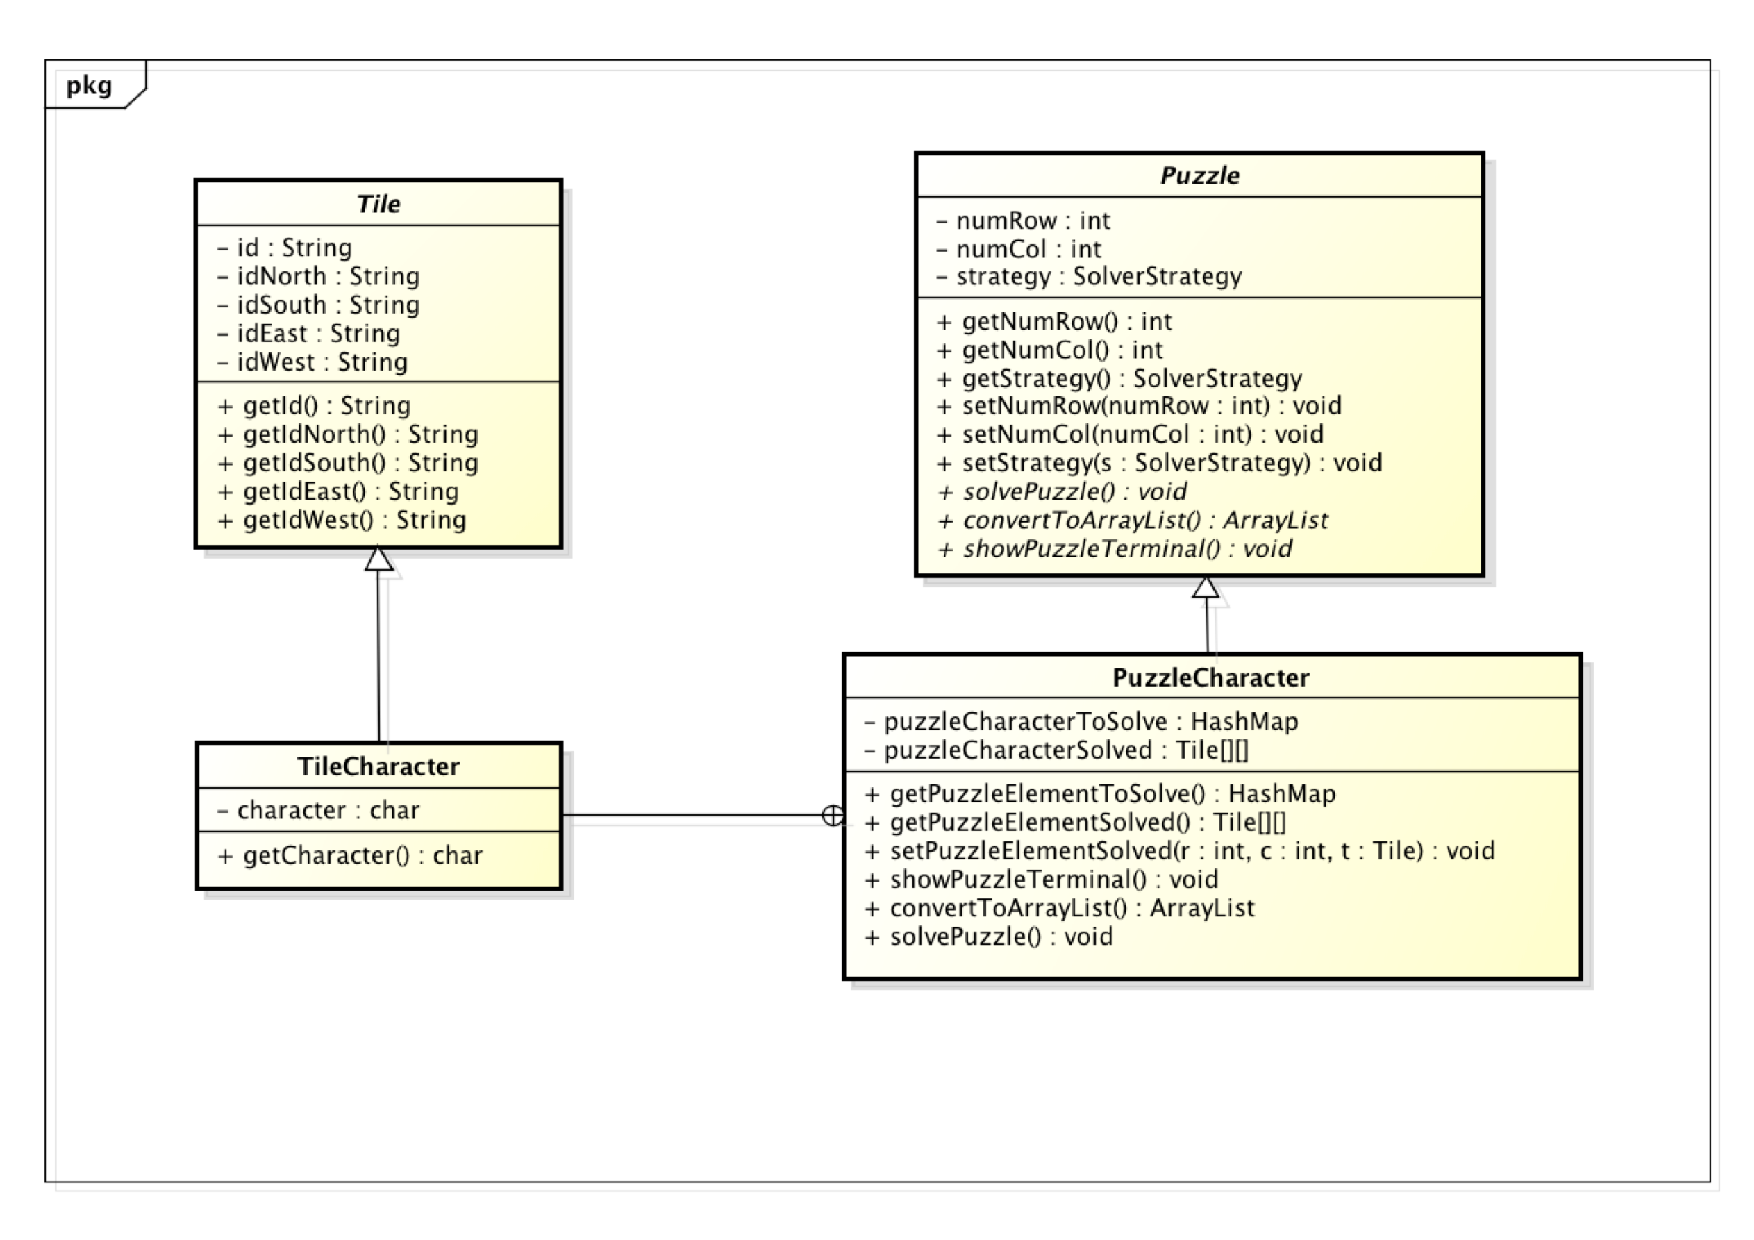
\includegraphics[width=15cm]{img/Puzzle.pdf}
			\caption{Package Puzzle}
			\label{Package Puzzle}
		\end{figure}

	\subsection{Package Solver}
Questo package contiente le classi che gestiscono la risoluzione del puzzle. \\
E' stato deciso di slegarla dal contesto strutturale del \textbf{Puzzle} in quanto svolgono due compiti logicamente diversi. Questo permette una più facile manutenibilità del codice e una maggiore possibilità di riutilizzo. \\
La presenza dell'interfaccia \textbf{SolverStrategy} permette la possibile implementazione di altri algoritmi di risoluzione senza andare a toccare le modalità introdotte nella classe \textbf{SolverAlgStrategy}. Sul client \textbf{PuzzleSolver} basterà cambiare l'algoritmo che si vorrà utilizzare. Questo, grazie al tentato utilizzo del design pattern Stratey, spiegato nel capitolo \textbf{\ref{DPS}}, sarà l'unico cambiamento da effettuare.
		\begin{figure}[htbp]
			\centering
			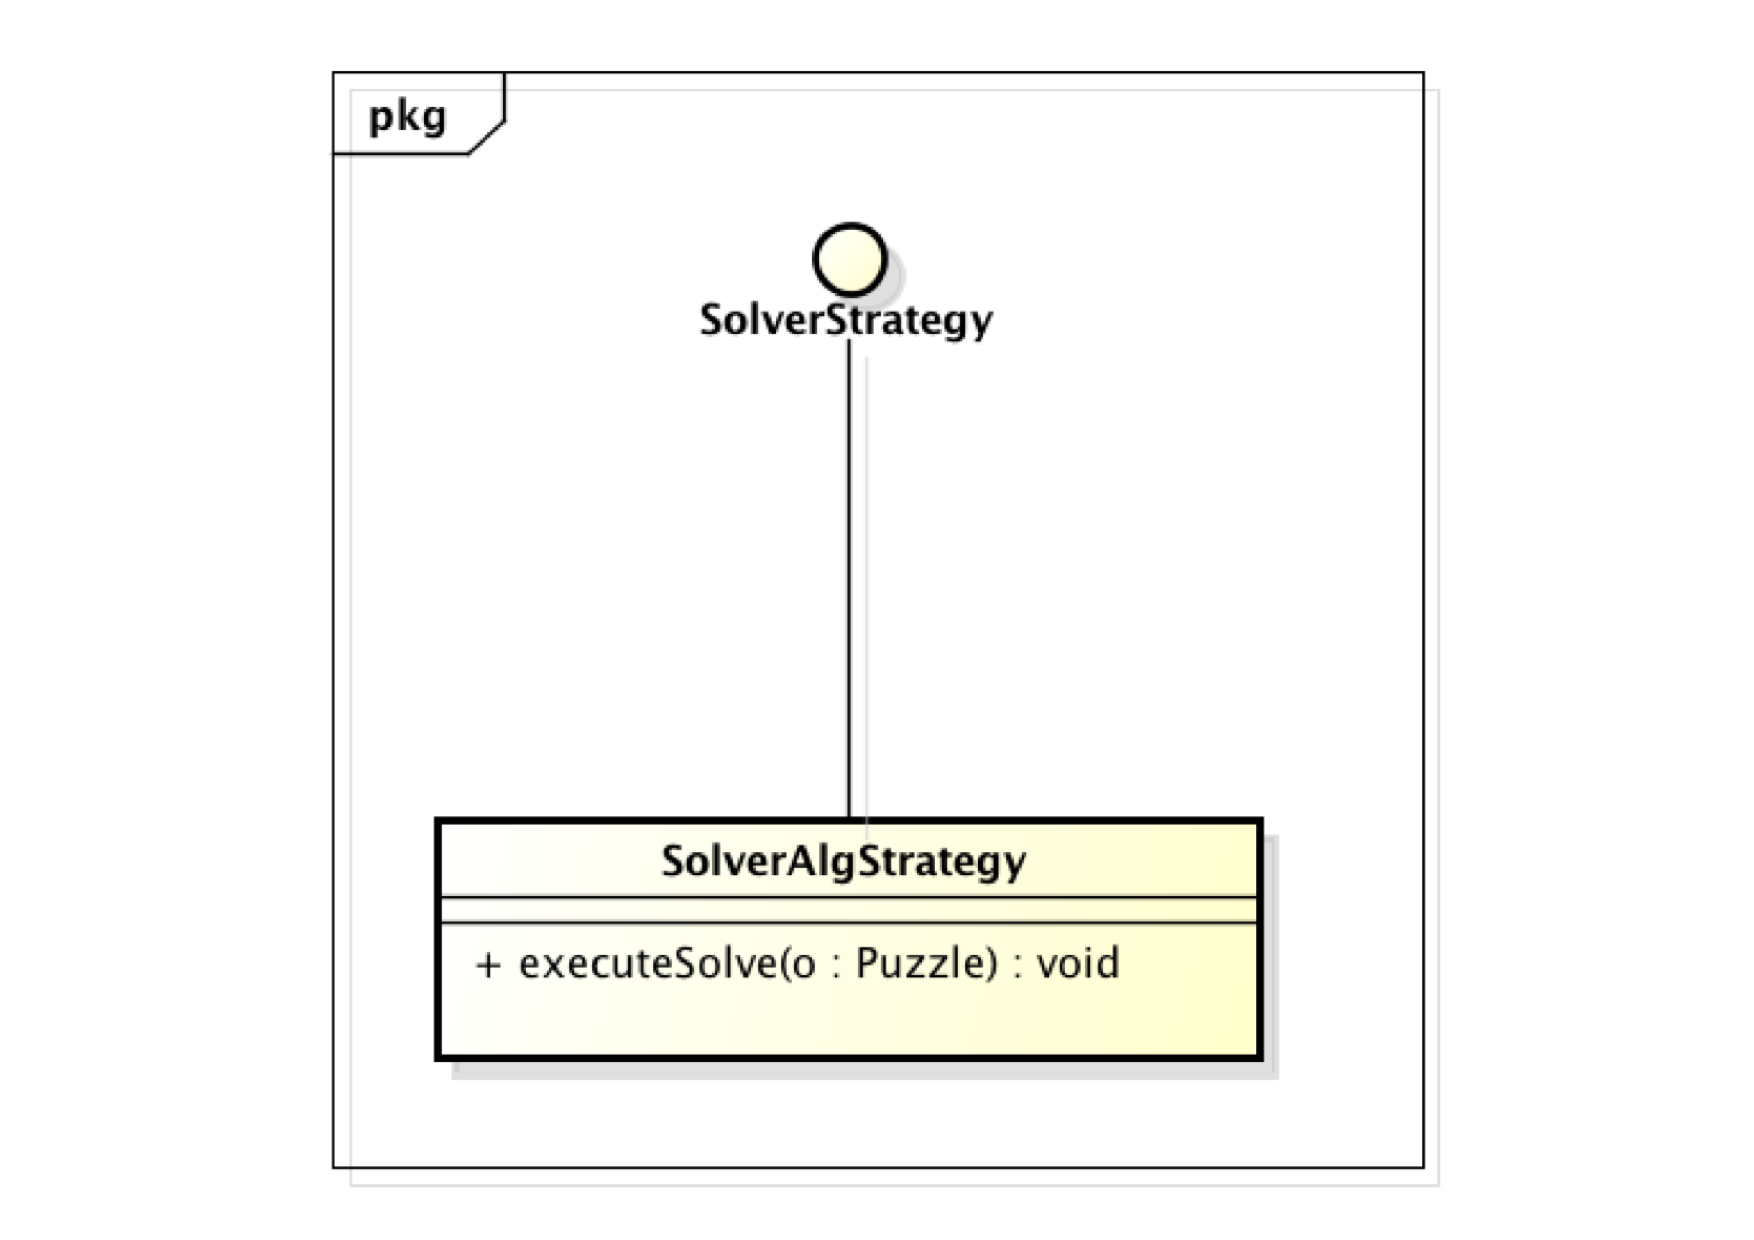
\includegraphics[width=15cm]{img/Solver.pdf}
			\caption{Package Solver}
			\label{Package Solver}
		\end{figure}
	
	\subsection{Package FileInputOutput}
Questo package contiene le classi necessarie a fare leggere un file in input e a scrivere il contenuto di qualcosa in un file in output. \\
Si è deciso di utilizzare un'interfaccia \textbf{FileIO} contenente il solo metodo \textbf{readContent} e non anche \textbf{writeContent} perché il primo ha una firma molto più generica e classica per la lettura di un file, permettendone così una ridefinizione in possibili sottoclassi future che potrebbero implementare un altro sistema per la lettura. \\
Essendo però \textbf{writeContent} più specifico per il problema del puzzle, si è deciso di tenerlo solo nella classe che implementa l'interfaccia.

		\begin{figure}[htbp]
			\centering
			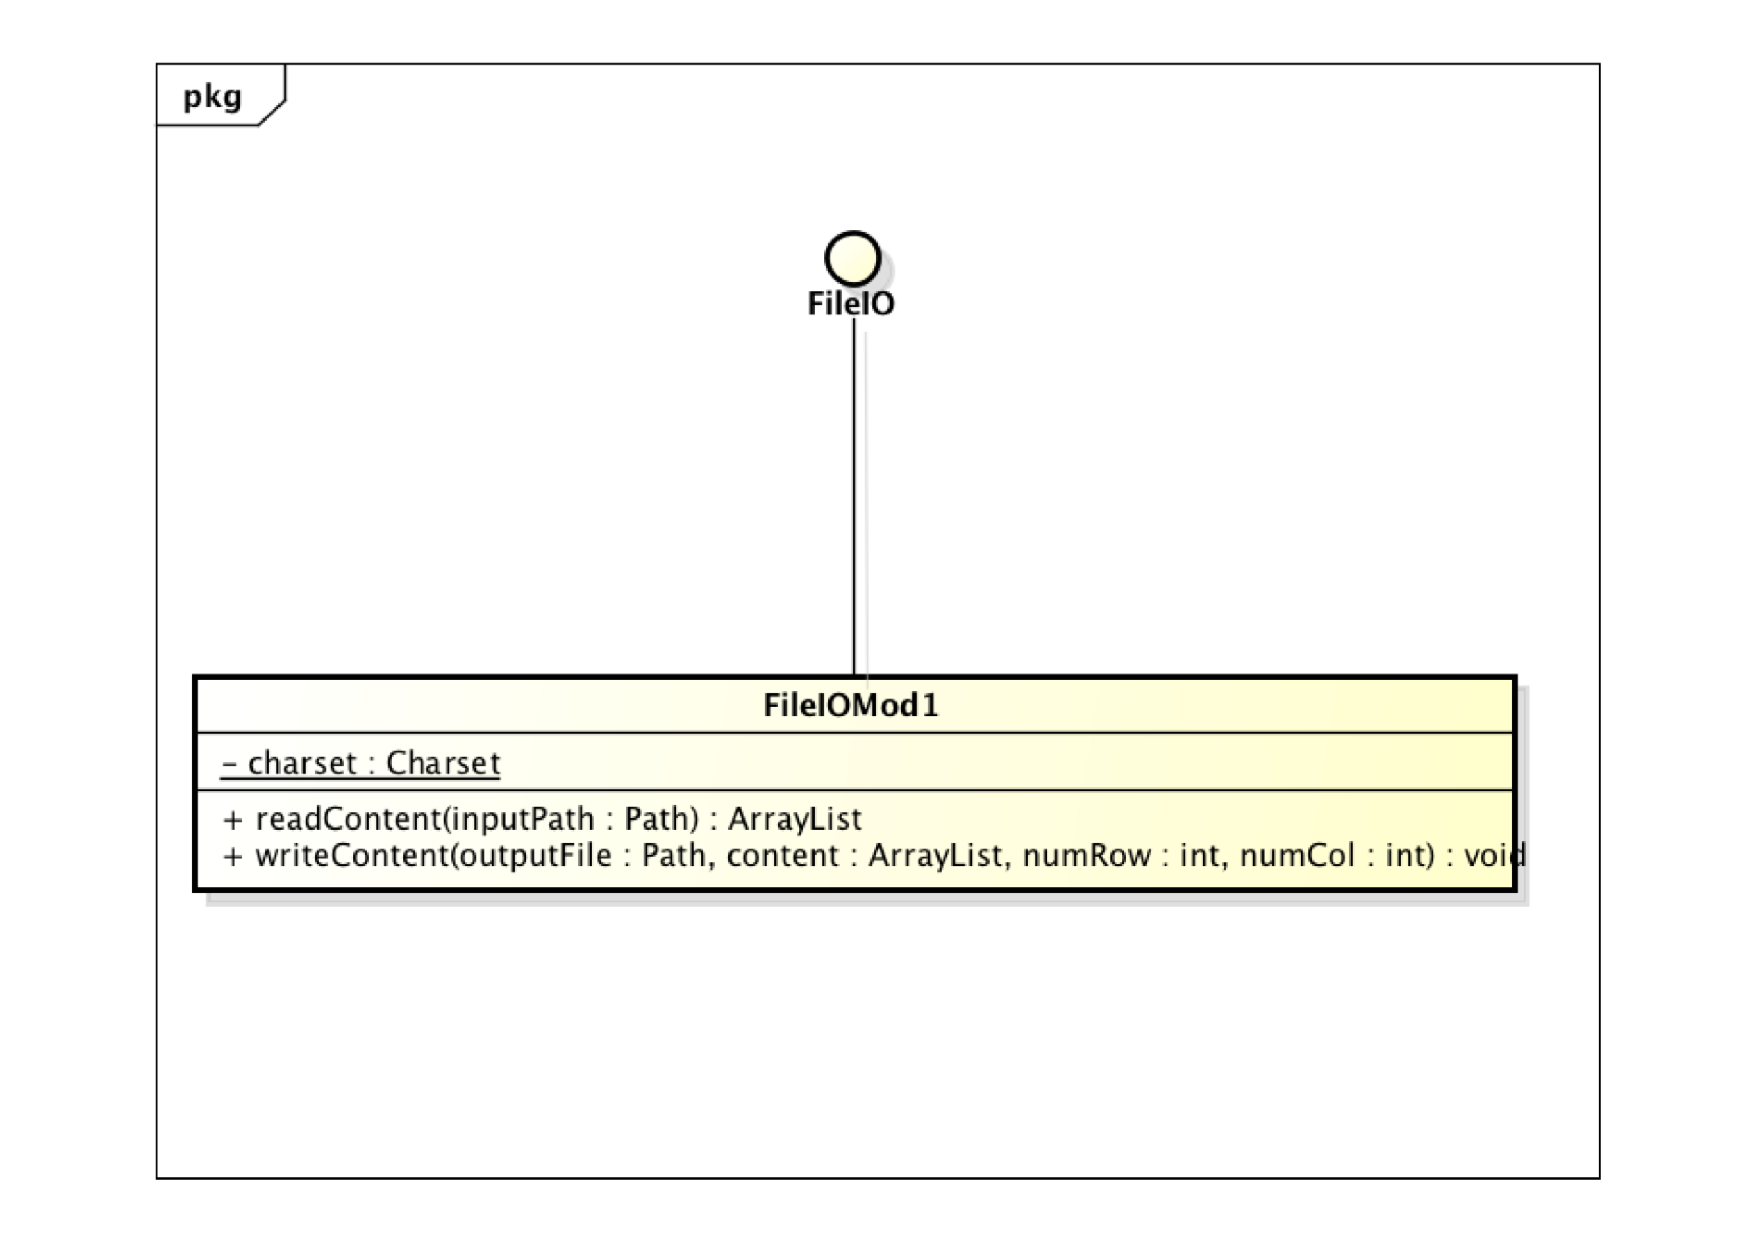
\includegraphics[width=15cm]{img/FileInputOutput.pdf}
			\caption{Package FileInputOutput}
			\label{Package FileInputOutput}
		\end{figure}

	
	\subsection{Design Pattern: Strategy} \label{DPS}
In questa sezione verrà esposto come si è cercato di implementare il desing pattern strategy tra \textbf{Solver} e \textbf{Puzzle}. \\
Si è scelto di utilizzarlo in quanto si possono avere molte implementazioni dell'algoritmo (alcune più efficienti di altre) e per garantire che la scelta di uno o di un altro non necessiti la ricodifica di una parte della classe \textbf{Puzzle}. \\
Seguendo la notazione espressa nel libro Design Patterns - Elementi per il riuso di software a oggetti di Gamma, Helm, Johnson, Vlissides viene illustrato il suo uso nel caso concreto del progetto. \\
\textbf{Partecipanti:}
		\begin{itemize}
			\item \textbf{Strategy} (SolverStrategy) :  dichiara un'interfaccia comune a tutti gli algoritmi supportati, nel nostro caso per ora solo uno. Context usa questa interfaccia per invocare l'algoritmo definito da un ConcreteStrategy;
			\item \textbf{ConcreteStrategy} (SolverAlgStrategy) : implementa l'algoritmo usando l'interfaccia Strategy;
			\item \textbf{Context} (Puzzle) : Contiene un riferimento a un oggetto Strategy. In particolare viene utilizzato il campo dati strategy. Viene configurato con un oggetto ConcreteStrategy; \\
		\end{itemize}
\noindent
\textbf{Collaborazioni:}
		\begin{itemize}
			\item Strategy e Context collaborano per implementare l'algoritmo voluto. Context passa se stesso come parametro ai metodi di Strategy. Questo consente a Strategy di invocare i metodi appropriati su Context;
			\item Context inoltra le richieste dai propri client verso Strategy.
		\end{itemize}
\noindent
	\begin{figure}[htbp]
		\centering
		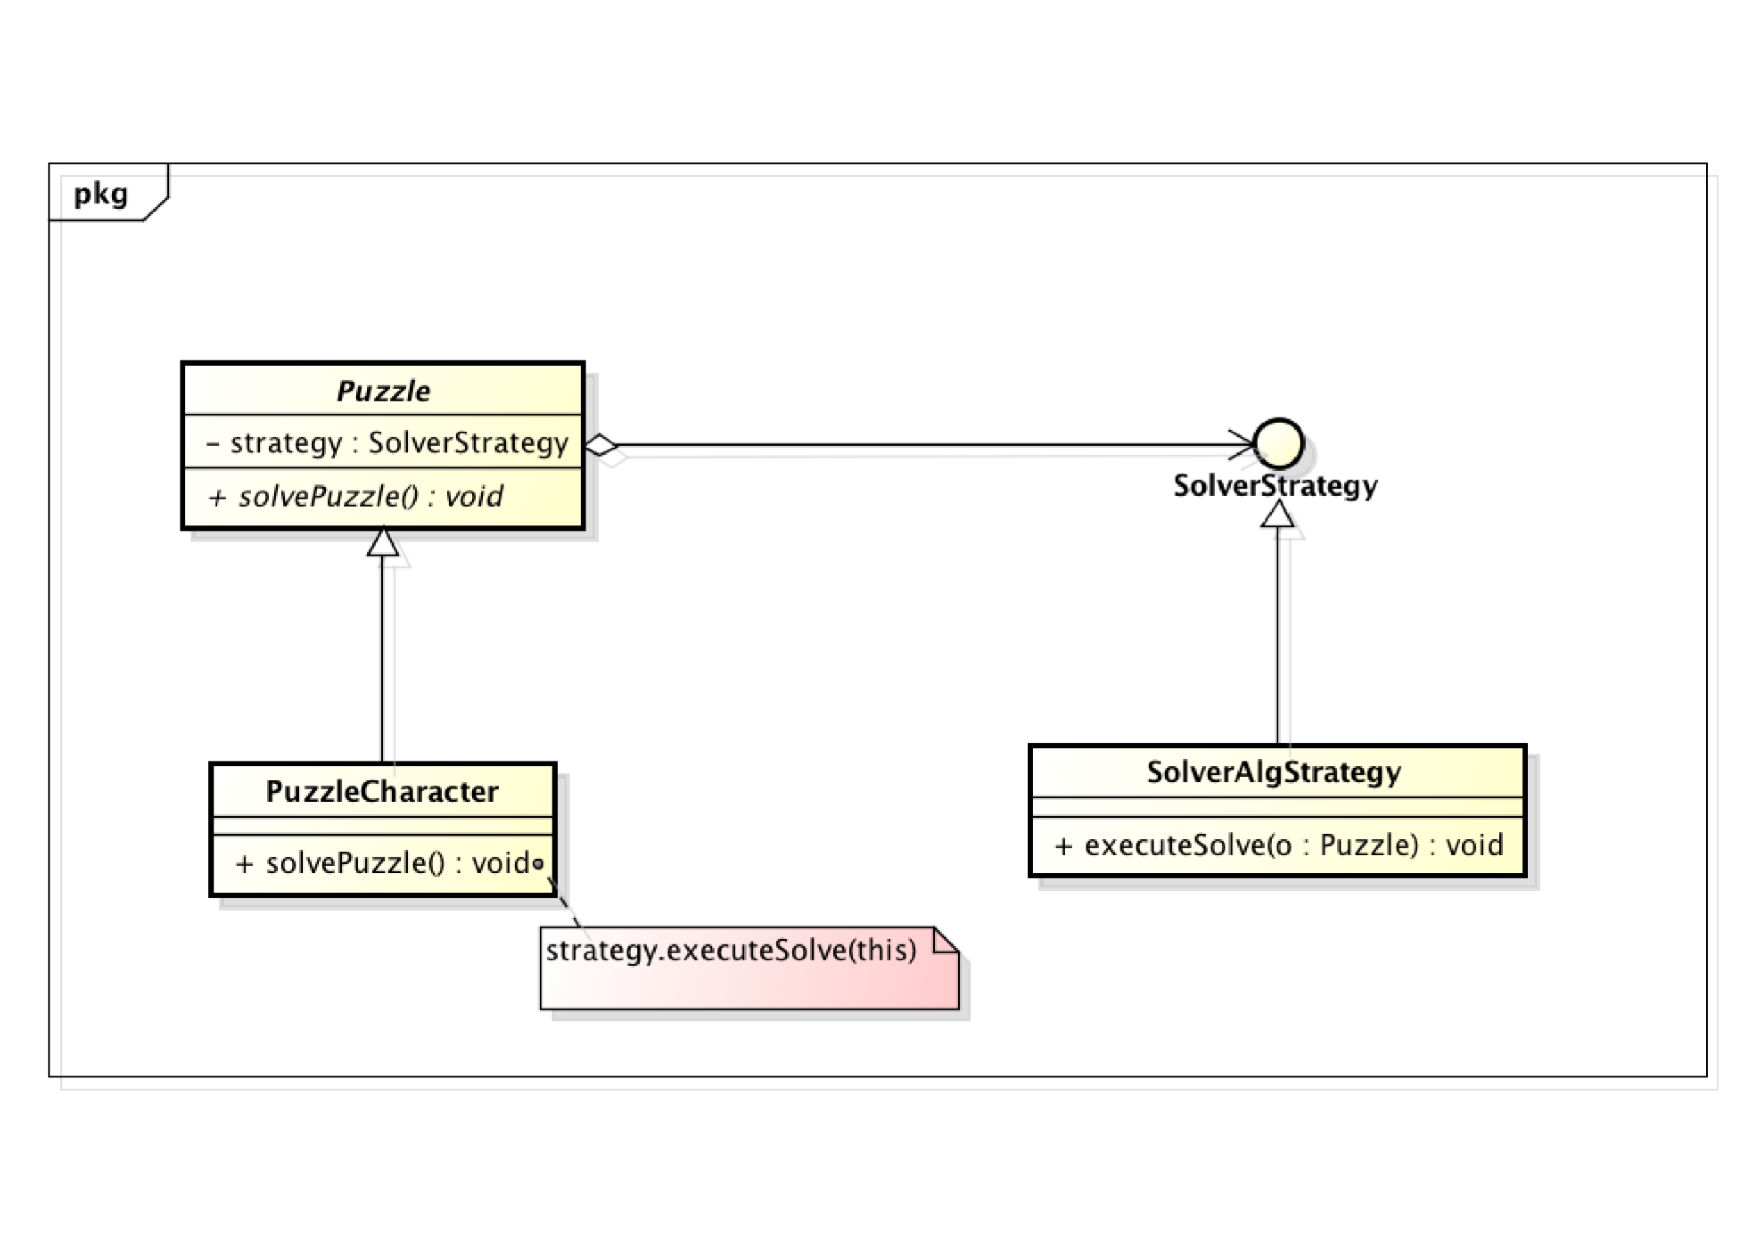
\includegraphics[width=15cm]{img/DesignPatternStrategy.pdf}
		\caption{Design Pattern Strategy}
		\label{Design Pattern Strategy}
	\end{figure}


